%!TEX root = Manuscript.tex

\chapter{Algorithmic and industrial context}
\label{chap:context}
\minitoc

\section{Industrial context}
\subsection{What is 5G ?}



Telecoms networks must manage more and more users while continually improving their bandwidth, latency and reliability. Nowadays, 4G is the standard deployed in most of the territory, and a new technology is under deployment: 5G. The term 5G defines a set of functional specifications. The organism that proposes these specifications is the ITU (International Telecommunication Union), an agency of the United Nation responsible for infromations and communications. For several years, the ITU-R (radiocommunication component of the ITU) has been working to determine the functional aspects that 5G must satisfy. Figure~\ref{fig:5gperf} from~\cite{dahlman20185g} illustrates some of those functional aspects, that ITU-R has formally referenced in IMT-2020 (the requirments of 4G are referenced as IMT-advanced): a bitrate up to 20Gbps ($\times 20$ compared to 4G), low end to end latencies down to 1ms ($10$ times lower than in 4G, we are focusing on this aspect in this thesis).
Also, 5G aims to offer an higher connection density (up to 1 million device$/km^2$), with an higher traffic capacity (from $0,1 Mbit/s/m^2$ in 4G to $10 Mbit/s/m^2$ in 5G) due to a larger uses of the spectrum. Others aspects as a better energy efficiency ($100$ times better in 5G than in 4G) or a better mobility are required. 

  \begin{figure}[h]
      \begin{center}
      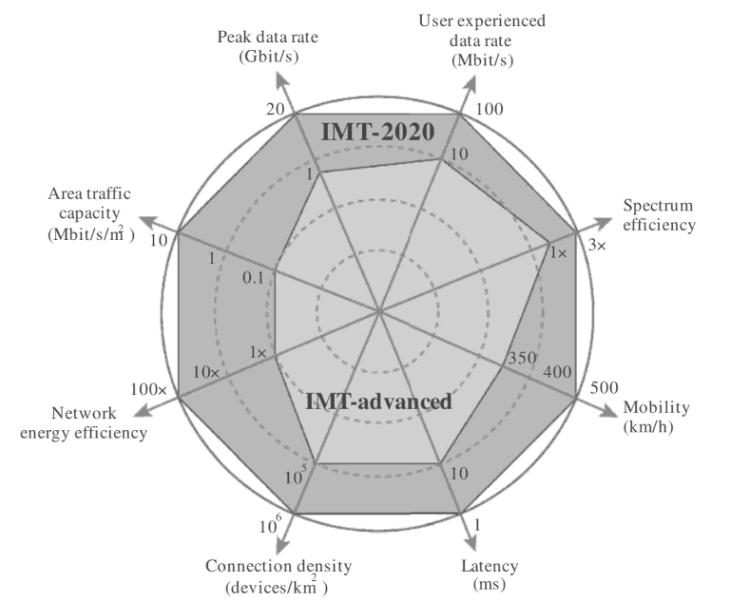
\includegraphics[width=1\textwidth]{Chapitre1/5Grequirements}
      \end{center}
      \caption{5G performances required by ITU-R}\label{fig:5gperf}
      \end{figure}

All these aspects lead us to various application cases. Figure~\ref{fig:usecases} taken from~\cite{5GACIA} establishes a non-exhaustive list of them, according to their different technical constraints. Indeed, low latency is required for applications like motion control that work in real time since one of the goals of 5G is to obtain dynamic programmable networks, for greater flexibility of use.
On the other hand, an higher bandwidth is usefull for applications like video streaming, augmented reality or ensuring the connectivity of a large number of terminals. By relaxing latency and bandwidth constraints, it is possible to expand further the number of devices (up to 1 million) for applications like sensors networks.

  \begin{figure}[h] 
      \begin{center}
      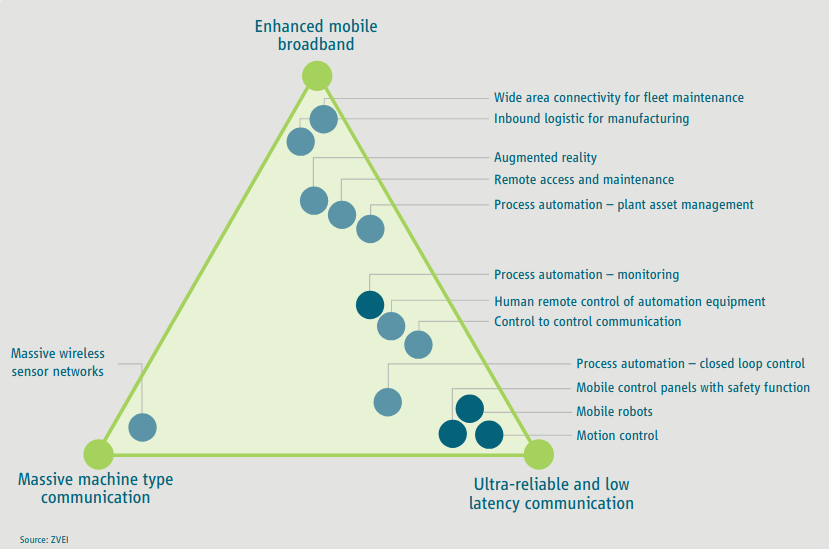
\includegraphics[width=1\textwidth]{Chapitre1/usecases.png}
      \end{center}
      \caption{Some examples of use cases for 5G}\label{fig:usecases}
      \end{figure}



\subsection{URLLC}


To meet these 5G functional specifications, the network equipments must follow some technical standards. The 3GPP (3rd Generation Partnership Project) is an union between several standard organizations which defines the technical specifications for 5G. 3GPP regulary publishes releases, that regroup new specifications. The first release focused on 5G was Release 15 (R15), released in 2018 \cite{RELEASENOKIA}.  

  \begin{figure}[h]
      \begin{center}
      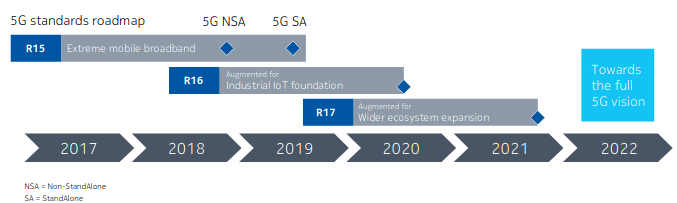
\includegraphics[width=1\textwidth]{Chapitre1/release.png}
      \end{center}
      \caption{3GPP releases 15, 16 and 17 calendar}\label{fig:release}
      \end{figure}
  
Release 15 focused on increasing throughput and interworking between 4G and 5G, and introduced the notion of URLLC (Ultra-Reliable Low-Latency Communication). Releases 16 an 17 have extended the notion of URLLC. The notion of URLLC consists in ensuring low packet loss and low latency communications. Indeed, several use cases (smart factories, control operations, \dots) needs some highly reliable communications in which the latency must be guaranteed. Current network managments does not ensure such constraints for all packets. 

\subsection{Statistical Multiplexing}


The expressed constraints expressed for low latency architectures and 5G standard are hard to met in current networks. In IP or even Ethernet networks, the traffic usually suffers of delay due to buffering. 

As we just mentioned, the current network nodes (routers for IP networks, switches for Ethernet networks) are not able to schedule packets. The only function of the nodes is to forward the packets to the right output port. If several flows have to use the same output port, then some packets can be put in a \textbf{buffer}, in order to wait the availability of the port \todo{figure}. 
The maximal bitrates of the links is thus dimentioned according to the use case. The bitrate is then calculated according to the average bitrate of the flows on the network and the cost of the links. The objective is to offer a good average quality of service for a minimal price. When a single input flow uses an ouput port, there is no issues. However, when several packets comming from several flows uses the same output port, we talk about \textbf{contention}, and the buffering induces additional latency for some packets of the flows. When there is too much packets in the buffer, the oldest packets of the buffer are \textbf{lost}. 

Such a technology ensures an easy deployment and managment of the networks and most of the time a good quality of service for a minimal cost for network providers, but it can induce some packet loss and high latencies. Hence, we talk about statistical multiplexing~\cite{krishnamurthy2003latency,venkatramani1994supporting}.

URLLC aims to ensure good end to end latency communications. To achieve such a goal, each component of the communication must satisfy a low latency: the radio communications, and the core network. This thesis focus on the core networks. 

\subsection{\textbf{R}adio \textbf{A}ccess \textbf{N}etwork}
To understand on which part of the network this thesis focuses on, we might describe how a radio access network works.

Current mobile network (aka cellular network) architecture consists in a distributed radio access networks: the mobile terminals connect to base stations (BTS for Base Transceiver Station as a generic name, eNB for evolved Node B in 3GPP LTE “4G” standard or gNB for 5G) that encompasses all the sub-systems needed to realize mobile communication~\cite{bouguen2012lte}. It mainly comprises the radio part, that furnishes the connection between the mobile terminal and the BTS, and the network part that provides control and management functions like mobility support (the main functionality being the support of handover from one BTS to another, i.e. the ability to pursue a communication when moving from range of an antenna to another).
The BTS are connected together by the Aggregation Network of the operator, itslef connected to the core network, in order to ensure communications with other operators RANs. Figure~\ref{fig:RAN} illustrates a communication between two mobiles using a different operator.

\begin{figure}
\begin{center}
\scalebox{0.4}{

\begin{tikzpicture}
  \SetGraphUnit{5}
    \tikzset{
  EdgeStyle/.append style = {->} }
   \tikzstyle{VertexStyle}=[shape = circle, draw, minimum size = 30pt]
 

  \node (p1) at (0,4) {
\includegraphics[width = 1cm]{phone.png}};
 
  \node (p2) at (0,2) {
\includegraphics[width = 1cm]{phone.png}};

  \node (p3) at (0,0) {
\includegraphics[width = 1cm]{phone.png}};
  
 \node (a1) at (7,1) {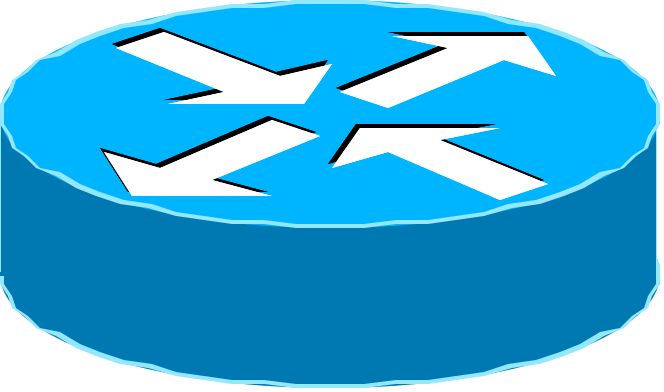
\includegraphics[width = 1cm]{switch.png}};
 \node (a2) at (7,3) {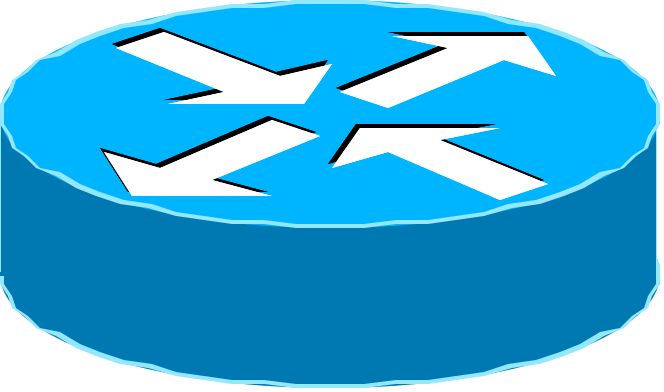
\includegraphics[width = 1cm]{switch.png}};
 \node (a3) at (9,1) {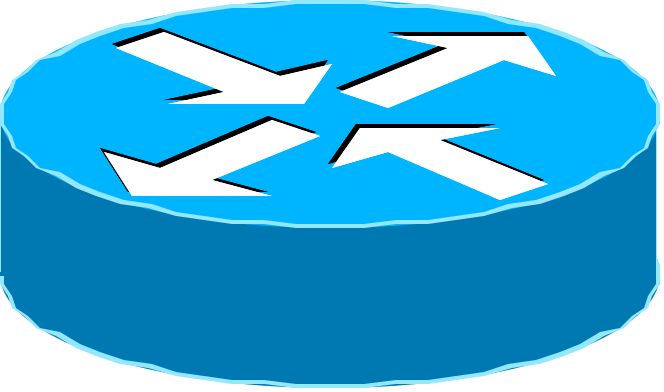
\includegraphics[width = 1cm]{switch.png}};
 \node (a4) at (9,3) {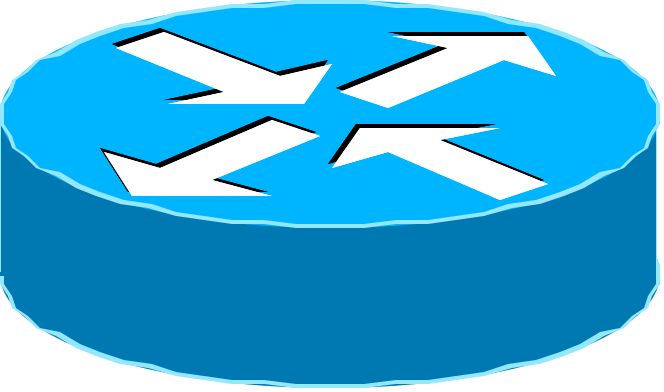
\includegraphics[width = 1cm]{switch.png}};

 \node (c1) at (12,3) {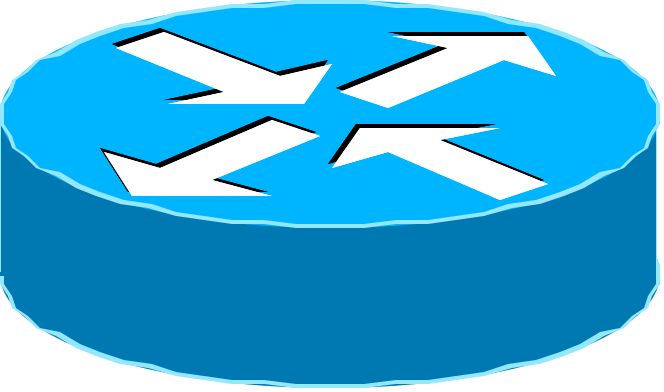
\includegraphics[width = 1cm]{switch.png}};
 \node (c2) at (12,5) {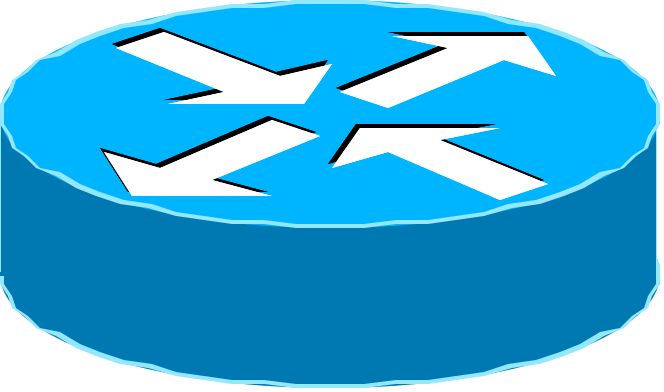
\includegraphics[width = 1cm]{switch.png}};
 \node (c3) at (14,3) {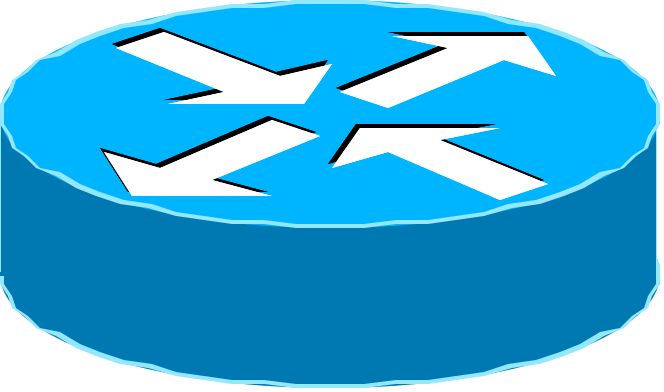
\includegraphics[width = 1cm]{switch.png}};
 \node (c4) at (14,5) {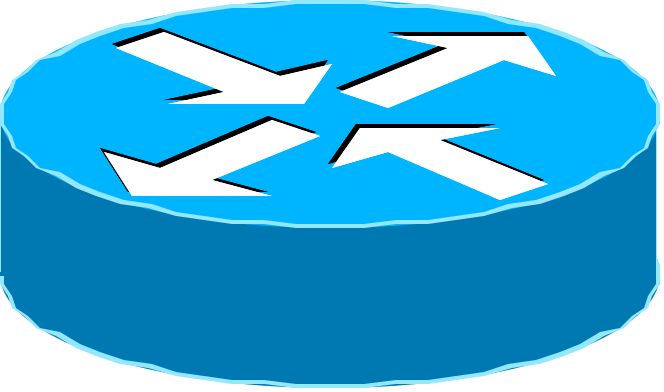
\includegraphics[width = 1cm]{switch.png}};

 \node (a5) at (17,1) {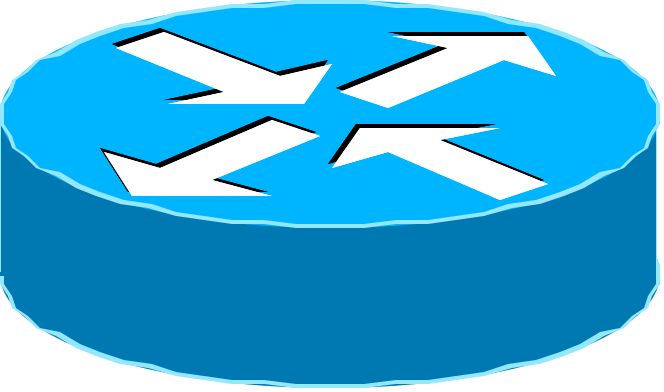
\includegraphics[width = 1cm]{switch.png}};
 \node (a6) at (17,3) {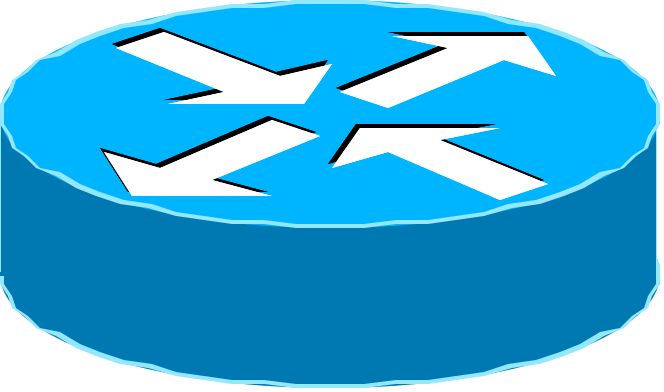
\includegraphics[width = 1cm]{switch.png}};
 \node (a7) at (19,1) {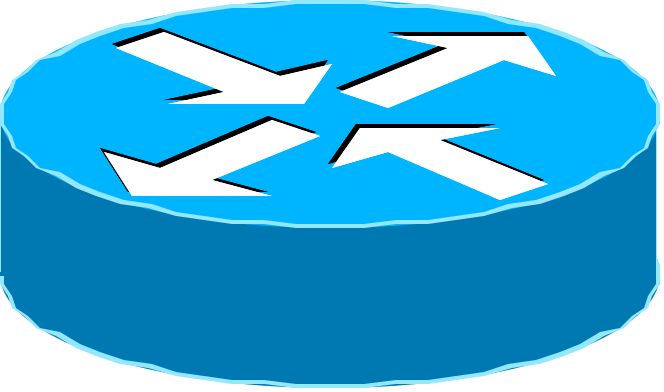
\includegraphics[width = 1cm]{switch.png}};
 \node (a8) at (19,3) {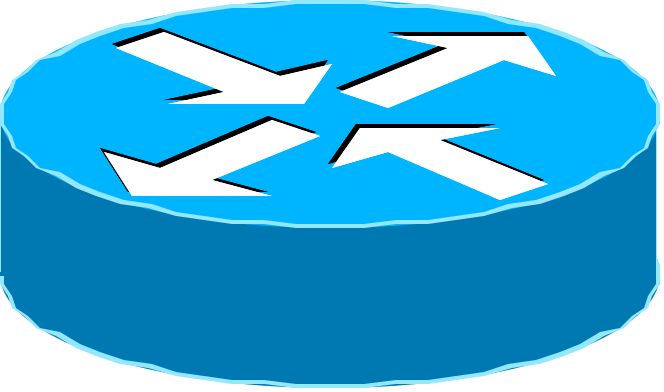
\includegraphics[width = 1cm]{switch.png}};


 \node (p4) at (26,4) {
\includegraphics[width = 1cm]{phone.png}};
 
  \node (p5) at (26,2) {
\includegraphics[width = 1cm]{phone.png}};

  \node (p6) at (26,0) {
\includegraphics[width = 1cm]{phone.png}};
  
   \node (r1) at (4,2) {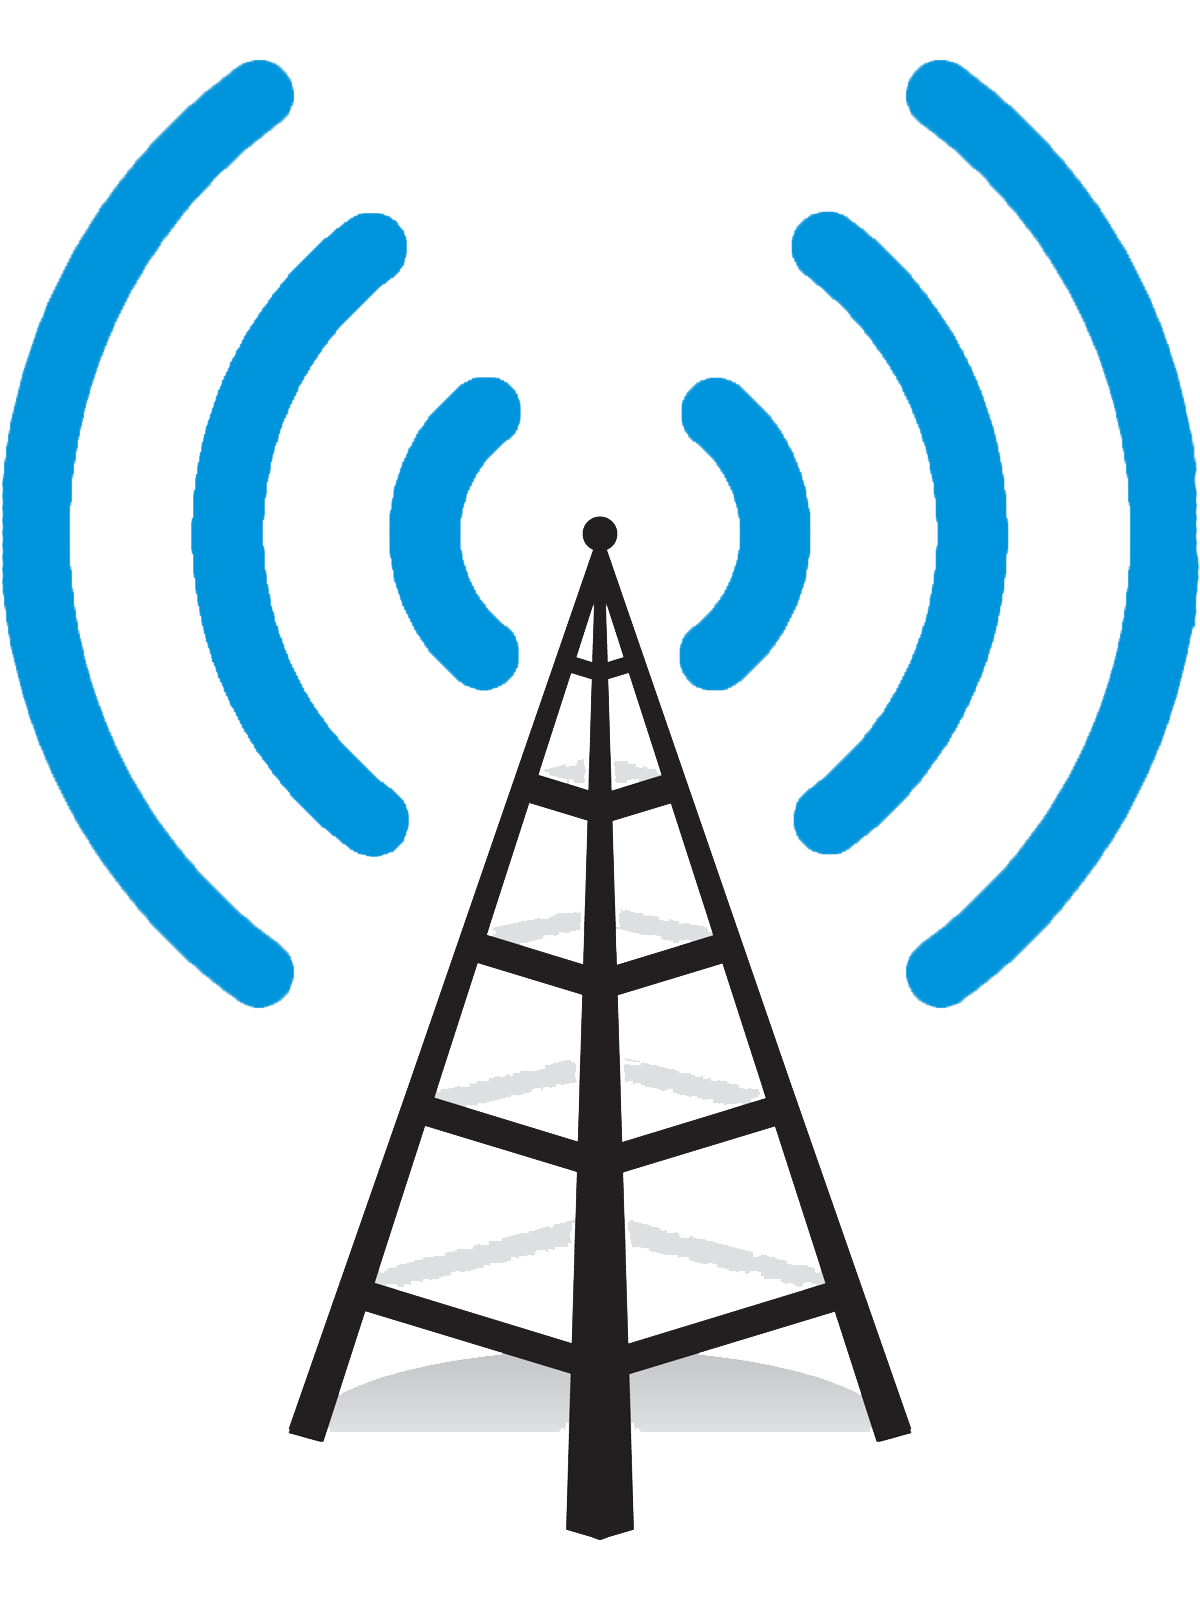
\includegraphics[width = 1cm]{rrh.png}};
   \node (r2) at (22,2) {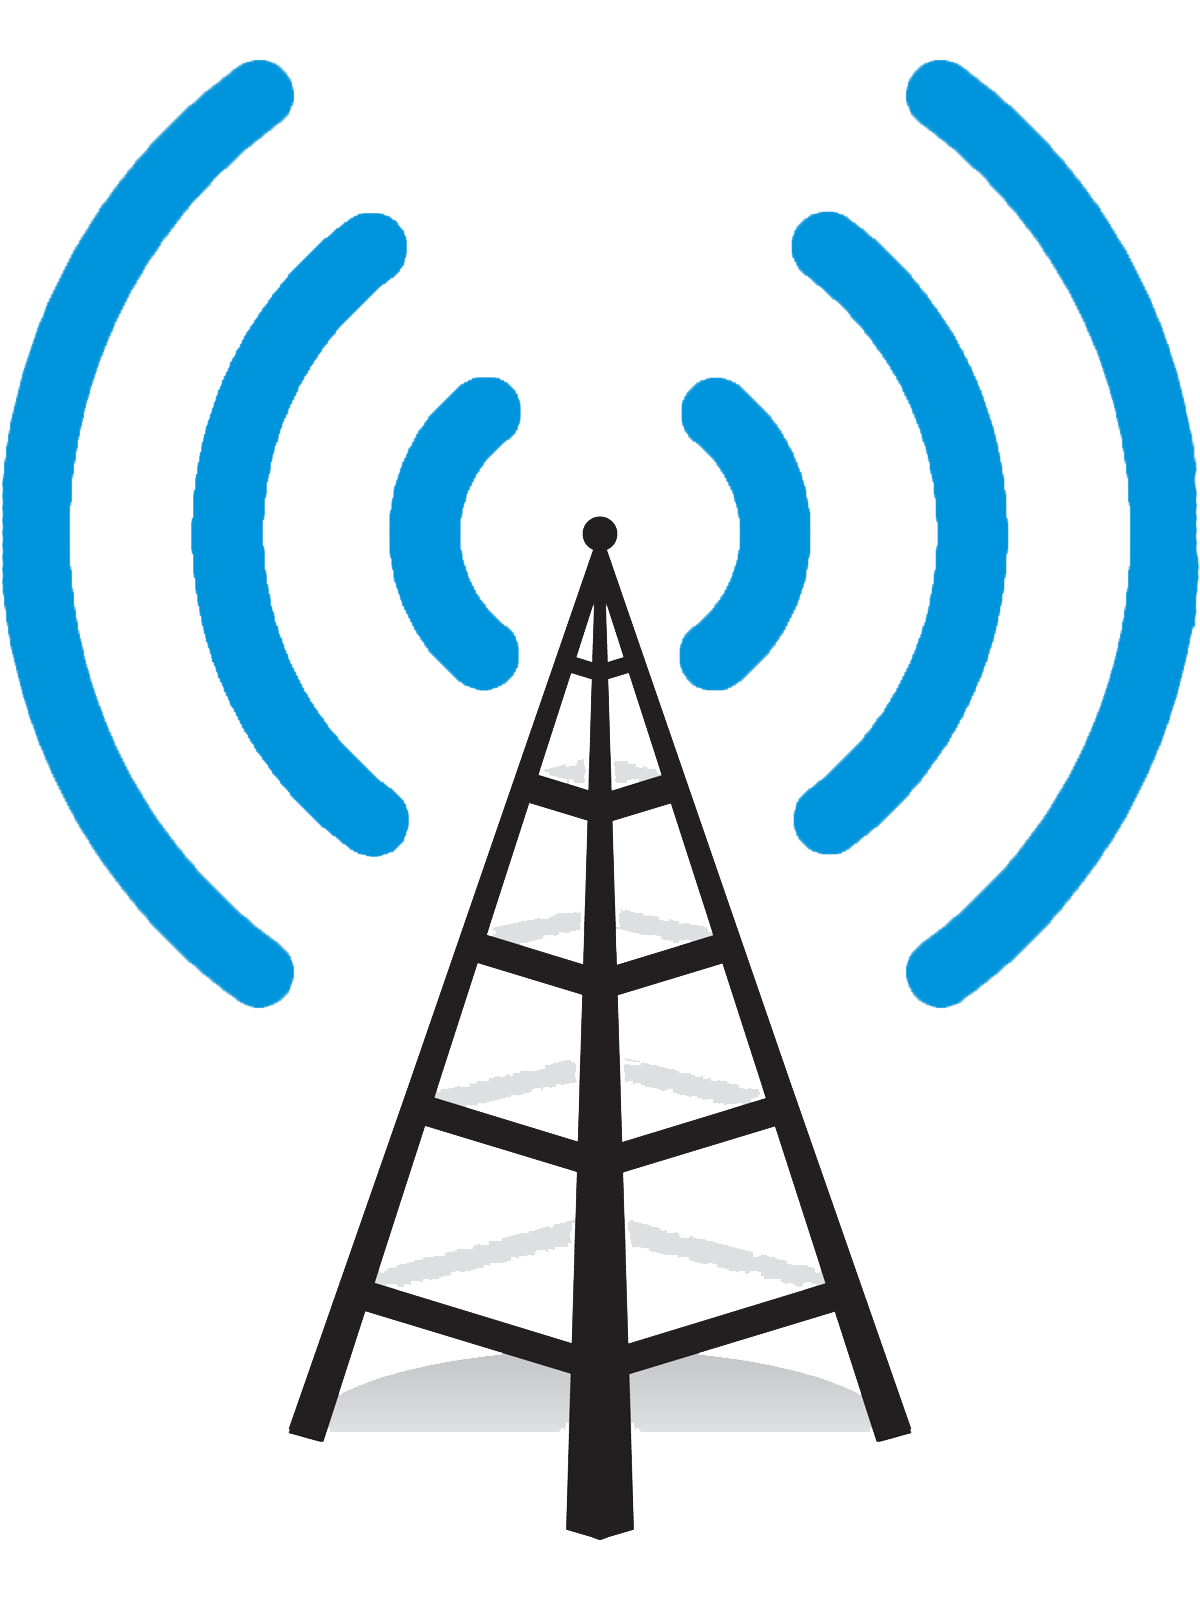
\includegraphics[width = 1cm]{rrh.png}};
   

 
\path (p1) edge [<->,color=red]  (r1);
\path (p2) edge [<->]  (r1);
\path (p3) edge [<->]  (r1);

\path (r1) edge [<->,color=red]  (a1);
\path (r1) edge [<->]  (a2);

\path (a1) edge [<->]  (a2);
\path (a3) edge [<->]  (a2);
\path (a4) edge [<->]  (a2);
\path (a3) edge [<->]  (a4);
\path (a3) edge [<->]  (a1);
\path (a4) edge [<->,color=red]  (a1);


\path (c1) edge [<->]  (c2);
\path (c3) edge [<->]  (c2);
\path (c4) edge [<->]  (c2);
\path (c3) edge [<->]  (c4);
\path (c3) edge [<->]  (c1);
\path (c4) edge [<->,color=red]  (c1);


\path (a5) edge [<->]  (a6);
\path (a7) edge [<->]  (a6);
\path (a8) edge [<->,color=red]  (a6);
\path (a7) edge [<->]  (a8);
\path (a7) edge [<->]  (a5);
\path (a8) edge [<->]  (a5);

 
\path (p4) edge [<->]  (r2);
\path (p5) edge [<->,color=red]  (r2);
\path (p6) edge [<->]  (r2);


\path (a4) edge [<->]  (c2);
\path (a3) edge [<->]  (c1);
\path (a3) edge [<->]  (c2);
\path (a4) edge [<->,color=red]  (c1);


\path (a6) edge [<->,color=red]  (c4);
\path (a5) edge [<->]  (c3);
\path (a5) edge [<->]  (c4);
\path (a6) edge [<->]  (c3);

\path (r2) edge [<->,color=red]  (a8);
\path (r2) edge [<->]  (a7);
\draw[dashed] (-1,-1) rectangle  (10,7);
\node at (5.5, 6.5) {\huge Operator $1$};
\node at (3, 4) {RAN};
\node at (8, 4) {Aggregation};

\draw[dashed] (16,-1) rectangle  (27,7);
\node at (22.5, 6.5) {\huge Operator $2$};
\node at (23, 4) {RAN};
\node at (18, 4) {Aggregation};

\draw[dashed] (11,2) rectangle  (15,7);
\node at (13, 6.5) {\huge Core};

\end{tikzpicture}
}




 \caption{An End to End communication between two mobiles.}

\label{fig:RAN}
\end{center}
\end{figure}


\subsubsection{Cloud RAN}
The evolutions proposed in next generations aim at evolving toward centralized radio network architectures (C-RAN, for Cloud Radio Access Network) to reduce consumption costs and power at the base stations~\cite{mobile2011c}. These C-RAN architectures include simplified base stations on the field. Depending on the architecture choice  
, it can be restricted to the radio part and the digital to analog conversion only. This can be identified by different names depending on the reference documents, including RU for Remote Unit or Remote Radio Heads (RRH). The later will be used the rest of the thesis. The other component of the C-RAN is composed of the processing units. One can distinguish tow levels of processing units: the DUs, for Distributed Units that are able to ensure a part of the computation tasks, and the CUs for Centralized Units that computes the most centralized tasks. In this thesis, we consider only CUs, that are also called BaseBand Units (BBU), we will use this term in the rest of the thesis. Those BBUs are located in the cloud. 

 \begin{figure}[h]
      \begin{center}
      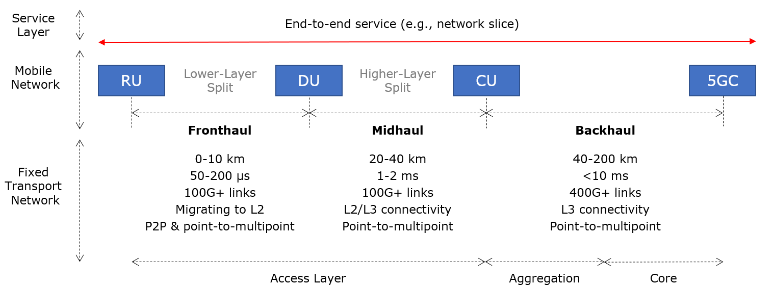
\includegraphics[width=1\textwidth]{Chapitre1/5gran.png}
      \end{center}
      \caption{Latency requirments depending of the communications between RRH (RU) and BBU (DU or CU) }\label{fig:5gran}
      \end{figure}

By cloud we define in the capability of instantiating executable programs in data centers that are transparently connected to the systems requiring the results of the program execution. The execution may be indifferently performed on virtualized machines, or bare metal one, or any other combinations. The network between RRH and BBU is called “Fronthaul Network”, or “Fronthaul” for short. Figure~\ref{fig:fronthaul} illustrates an example of fronthaul in which several BBU are gathered in a same datacenter. 

  \begin{figure}[h]
      \begin{center}
      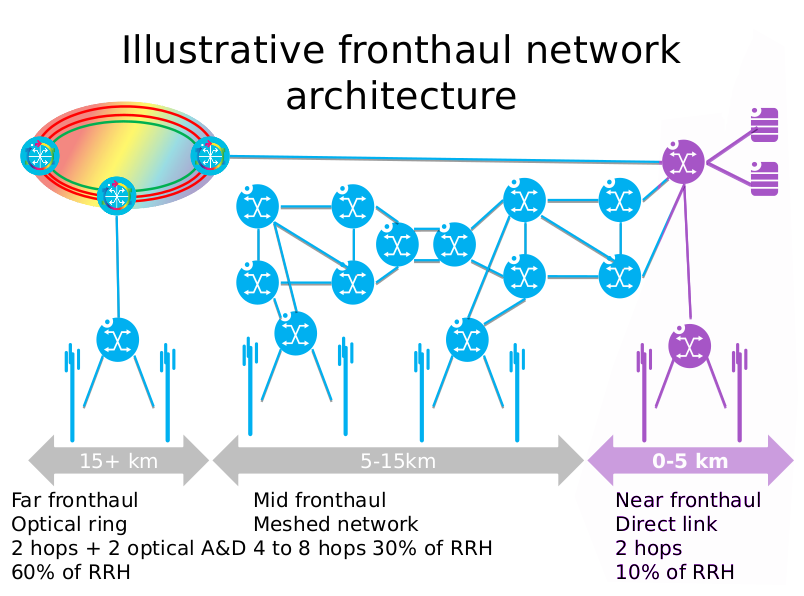
\includegraphics[width=1\textwidth]{Chapitre1/fronthaul.png}
      \end{center}
      \caption{An example of fronthaul network for Clound RAN}\label{fig:fronthaul}
      \end{figure}
      
      \subsubsection{Split}

      As mentioned above, in C-RAN, most of the computation tasks of the BTS must be centralized on the BBU. There are several components that can be centralized, but the more we centralize the ressources, the higher are the latency constraints.
      Figure~\ref{fig:CRANsplit} illustrates the two different ways proposed to split the BTS. The first one, called ``Full centralization'' leaves only the radio functions to the RRH, while the second one, called ``partial centralization'', keeps the baseband processing function into the RRH. The works presented in this thesis allow to send an high amount of data in the network while minimizing latency. Such a model matches with the first split, this is why we talk about BaseBand Units (BBU) here.
      
   \begin{figure}[h]
      \begin{center}
      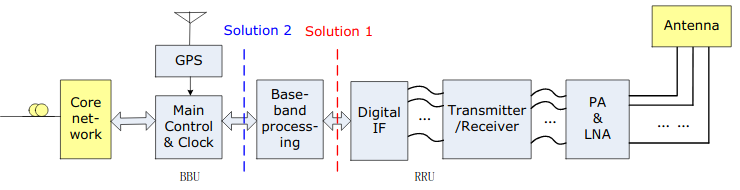
\includegraphics[width=1\textwidth]{Chapitre1/CRANsplit.png}
      \end{center}
      \caption{The two different split for Cloud-RAN}\label{fig:CRANsplit}
      \end{figure}
      \begin{figure}[h]
      \begin{center}
      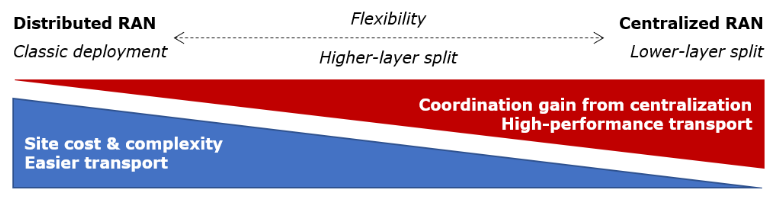
\includegraphics[width=1\textwidth]{Chapitre1/flexibility.png}
      \end{center}
      \caption{The more centralized is the RAN, the hardest is the transport and the lowest is the cost of coordination for the antennas}\label{fig:flexibility}
      \end{figure}
       
This kind of architecture faces the challenge of mastering the latency in the transfer process between the RRHs on the field and BBUs in the cloud. Low latency is already critical for the deployment of C-RAN approach in LTE “4G” networks. The standard requires hard time constraints for functions like HARQ (Hybrid Automatic Repeat reQuest) that needs to be processed in less than $3ms$ \cite{bouguen2012lte}. Considering processing time into the BBU, the time budget over the network can be as low as $400\mu s$ for a round trip. One specificity in this C-RAN context is not only the latency constraint, but also the periodicity of the data transfer between RRH and BBU (this HARQ constraint must be enforced for each frame emitted every millisecond). Looking beyond current mobile network generation, one must have in mind that ongoing 5G standards will require to reach end-to-end expected latency as low as $1ms$ (depending on targeted services)~\cite{boccardi2014five}. New scheduling and new technologies have to be considered to guarantee delay constrained periodic data transfers. 


\subsection{Technical solution for low latency}
Statistical multiplexing was the trend packet based netwoks in the last $40$ years, but it is not adapted to our context since they can not provide latency constraints \cite{khaunte2003technique}. If they can be used to prioritize some packets over the others (e.g. Express Forwarding against Best Effort), they fail to ensure delivery of a given packet in a given time delay when several packets compete for the same resource. 
The best current solution is to rely on an almost full optical approach, where each end-points (RRH on one side, BBU on the other side) are connected through direct fiber or full optical switches \cite{leclerc2016transmission}\cite{leclerc2016signaling}. This architecture is very expensive and hardly scales in the case of a mobile network. As illustrative purpose, a single (one operator) mobile network in France is composed of about $10,000$ base stations. This number will increase by a factor of $2$ to $20$ with the emergence of “small cells” that allow increasing base station density and to reach higher throughput \cite{leclerc2016transmission}\cite{leclerc2016signaling}. It is then needed to find a solution to offer low latency over commoditized packet based networks. 

Although 3GPP standards for 5G are not completely frozen yet, the core networks should use ethernet technology. Time Sensitive Networking (TSN) is a task group of IEEE that develop some standards in ethernet. The standard we focus here is 802.1Qbv \cite{ieee802}  
  
802.1Qbv allows us to manage the flows in the nodes by a gate mechanism. Knowing the routing over the network, it is possible to schedule on each node the time at which a flow must be sent by the node on each link in order to prioritize the most critical flows. The scheduler sends a  GCL (Gate Control List) to the node. 
Figure~\ref{fig:tsnqbv} found in \cite{durr2016no} shows the mechanism of a switch with the 802.1Qbv technology. Considering a given period ($T_{cycle}$ in the figure), the switch select at each times ($T_1 , T_2 , \ldots$ the queues that must be open to transmit packets. In figure 6, at time $T_1$, all gates exept the one for scheduled traffic are open, at time $T_2$, all gates are closed and at time $T_3$ only the gate for scheduled traffic is open.
  \begin{figure}[h]
      \begin{center}
      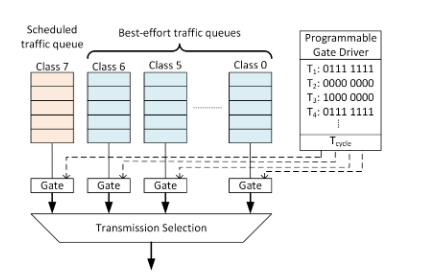
\includegraphics[width=0.8\textwidth]{Chapitre1/tsnqbv.png}
      \end{center}
      \caption{IEEE 802.1Qbv mechanism}\label{fig:tsnqbv}
      \end{figure}
      
Such a mechanism leads us to determine the GCL in order to let the C-RAN flows cross the nodes at the exact time they arrive. Furthermore, it is essential to schedule the different C-RAN flows so that two flows never use the same resource at the same time.
   
   \todo{meilleure conclusion qui reprends tout et explique ce qu'est notre pb + expliquer bien la periodicité}
\section{Algorithmic related works}

  We show in this article that statistical multiplexing, even in a fronthaul network with a small load, does not comply with the latency requirements of C-RAN. Therefore, current solutions~\cite{pizzinat2015things,tayq2017real}  use dedicated circuits for the fronthaul. Each end-point (RRH on one side, BBU on the other side) is connected through direct fiber or full optical switches. This architecture is very expensive and hardly scales in the case of a mobile network composed of about $10,000$ base stations. The deterministic approach we propose has gained some traction recently: Deterministic Networking is under standardization in IEEE 802.1 TSN group~\cite{finn-detnet-architecture-08}, as well at IETF DetNet working group~\cite{ieee802}. Several patents on concepts and mechanisms for DetNet have been already published, see for example~\cite{howe2005time,leclerc2016transmission}. 
     
The algorithmic problem we focus on may look like wormhole problems~\cite{cole1996benefit}, but we want to minimize the time lost in buffers and not just to avoid deadlocks. Several graph colorings have been introduced to model similar problems such as the allocation of frequencies~\cite{borndorfer1998frequency}, bandwidths~\cite{erlebach2001complexity} or routes~\cite{cole1996benefit} in a network. Unfortunately, they do not take into account the periodicity of the scheduling and the associated problems are already $\NP$-complete. The only coloring with periodicity is the circular coloring~\cite{zhou2013multiple} but it is not expressive enough to capture our problem. 
The problem \pall on a star routed network is very close to a two flow-shop scheduling problem~\cite{yu2004minimizing} with the additional constraint of periodicity. To our knowledge, all studied periodic scheduling problems are different from \pall that we consider in this article. 
Either the aim is to minimize the number of processors on which the periodic tasks are scheduled~\cite{korst1991periodic,hanen1993cyclic} while our problem correspond to a single processor and a constraint similar to makespan minimization. Or, in cyclic scheduling~\cite{levner2010complexity}, the aim is to minimize the period of a scheduling to maximize the throughput, while our period is fixed. 

The train timetabling problem~\cite{lusby2011railway} and its restriction, the periodic event scheduling problem~\cite{serafini1989mathematical} are generalizations of our problem. Indeed, they take the period as input and can express the fact that two trains (like two messages) should not cross. However, they are much more general: the trains can vary in size, speed, the network can be more complex than a single track and there are precedence constraints. Hence, the numerous variants of train scheduling problems are very hard to solve (and always $\NP$-hard). Thus, some delay is allowed to make the problems solvable and most of the research done~\cite{lusby2011railway} is devising practical algorithms using branch and bound, mixed integer programming, genetic algorithms\dots  In the same spirit, complex scheduling problems for time sensitive networks have also been practically solved, using mixed integer programming~\cite{nayak2017incremental,steiner2018traffic} or an SMT solver~\cite{dos2019tsnsched}.



Expliquer la litérature, et ce qui diffère de notre pb à nous